\chapter{Diseño e Implementación} % Main chapter title

\label{Chapter3} % Change X to a consecutive number; for referencing this chapter elsewhere, use \ref{ChapterX}
\definecolor{mygreen}{rgb}{0,0.6,0}
\definecolor{mygray}{rgb}{0.5,0.5,0.5}
\definecolor{mymauve}{rgb}{0.58,0,0.82}

\lstset{ %
  backgroundcolor=\color{white},   % choose the background color; you must add \usepackage{color} or \usepackage{xcolor}
  basicstyle=\large,        % the size of the fonts that are used for the code
  breakatwhitespace=false,         % sets if automatic breaks should only happen at whitespace
  breaklines=true,                 % sets automatic line breaking
  captionpos=b,                    % sets the caption-position to bottom
  commentstyle=\color{mygreen},    % comment style
  deletekeywords={...},            % if you want to delete keywords from the given language
  %escapeinside={\%*}{*)},          % if you want to add LaTeX within your code
  %extendedchars=true,              % lets you use non-ASCII characters; for 8-bits encodings only, does not work with UTF-8
  %frame=single,	                   % adds a frame around the code
  keepspaces=true,                 % keeps spaces in text, useful for keeping indentation of code (possibly needs columns=flexible)
  keywordstyle=\color{blue},       % keyword style
  language=[ANSI]C,					% the language of the code
  %otherkeywords={*,...},           % if you want to add more keywords to the set
  numbers=none,                    % where to put the line-numbers; possible values are (none, left, right)
  numbersep=5pt,                   % how far the line-numbers are from the code
  numberstyle=\tiny\color{mygray}, % the style that is used for the line-numbers
  rulecolor=\color{black},         % if not set, the frame-color may be changed on line-breaks within not-black text (e.g. comments (green here))
  showspaces=false,                % show spaces everywhere adding particular underscores; it overrides 'showstringspaces'
  showstringspaces=false,          % underline spaces within strings only
  showtabs=false,                  % show tabs within strings adding particular underscores
  stepnumber=1,                    % the step between two line-numbers. If it's 1, each line will be numbered
  stringstyle=\color{mymauve},     % string literal style
  tabsize=2,	                   % sets default tabsize to 2 spaces
  title=\lstname,                   % show the filename of files included with \lstinputlisting; also try caption instead of title
  morecomment=[s]{/*}{*/},%
  literate=%
}

En este capítulo se presenta la arquitectura del \textit{firmware} y el patrón de diseño usado para los módulos del sistema.  Asimismo, se detallan aspectos funciones de cada módulo y se fundamentan las elecciones de los distintos componentes de hardware utilizados.

%----------------------------------------------------------------------------------------
%	SECTION 1
%----------------------------------------------------------------------------------------
\section{Diseño de módulos y definición de interfaces}
\label{sec:modulos}

Se optó por un diseño fuertemente modularizado en archivos, junto a un modelo de capas jerárquicas para organizar el código en distintos niveles de abstracción.

En la figura \ref{fig:capas} se pueden observar, agrupadas por color, las capas utilizadas en este trabajo.  En color amarillo, el paquete de drivers provistos por el fabricante del silicio; en color naranja la capa de bibiotecas; la capa de abstracción de \textit{hardware} (HAL, por sus siglas en inglés) en color verde; y finalmente, en color celeste, la capa de aplicación con los cuatro módulos implementados.

%\vspace{10px}

\begin{figure}[ht]
	\centering
	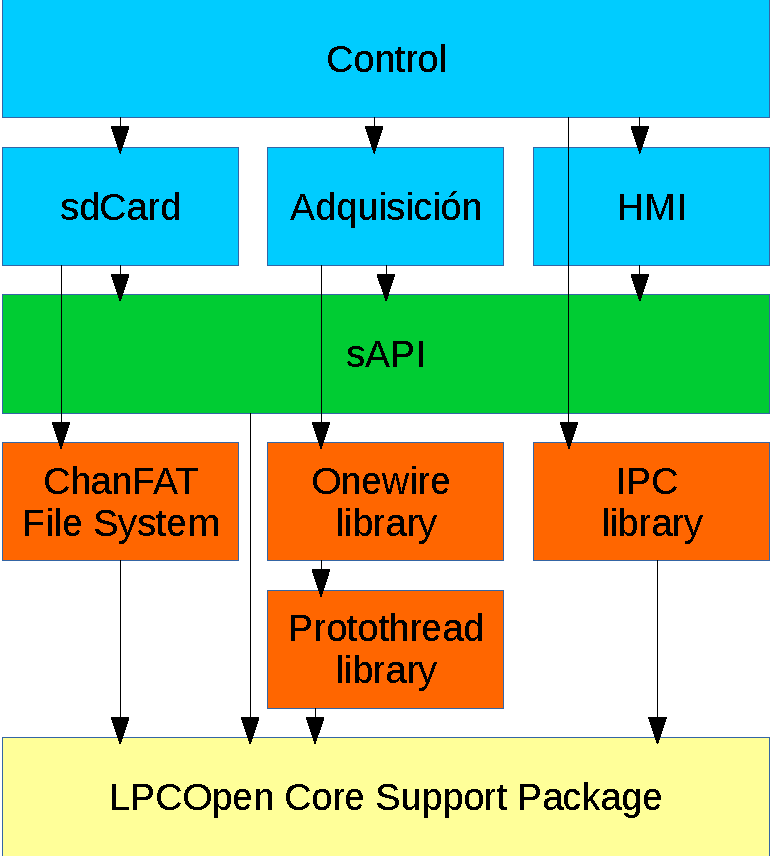
\includegraphics[width=.55\textwidth]{./Figures/capas.pdf}
	\caption[Estructura de capas para el \textit{firmware}.]{Estructura de capas para el \textit{firmware}. En orden creciente de nivel de abstracción: \textit{core support package} (amarillo), bibliotecas (naranja), sAPI (verde) y la capa de aplicación (celeste) con los 4 módulos implementados.}
	\label{fig:capas}
\end{figure}

\vspace{10px}

Para los módulos en la capa de aplicación, se confeccionó una matriz de trazabilidad de los requerimientos referidos al firmware, detallados en la sección \ref{sec:requerimientos}.

La tabla \ref{tab:trazabilidad} permite saber en qué módulo del firmware serán implementados los requerimientos funcionales del proyecto.  Asimismo, permite controlar que todo este subconjunto de requerimientos sea implementado y que no haya superposición entre la funcionalidad de cada módulo.

\vspace{5px}

\begin{table}[ht]
\centering
\caption[Matriz de trazabilidad de requerimientos funcionales]{Matriz de trazabilidad de requerimientos funcionales con los módulos de \textit{firmware}}
\label{tab:trazabilidad}
\begin{tabular}{lcccc}
\toprule
\textbf{Requerimiento} & \textbf{Control} & \textbf{sdCard} & \textbf{Adquisición} & \textbf{HMI} \\ \midrule
2.1 Adquirir temperatura                   &                  &                 & X                    &              \\ %\hline
2.2 Adquirir velocidad de viento           &                  &                 & X                    &              \\ %\hline
2.3 Almacenar datos                        &                  & X               &                      &              \\ %\hline
2.4 Perfiles de consumo                    & X                &                 &                      &              \\ %\hline
2.5 Interfaz                               &                  &                 &                      & X            \\ \bottomrule
\end{tabular}
\end{table}

Se definió un nuevo tipo de dato, \texttt{module\_t} que contiene campos de control para los módulos. Se observa su definición en el algoritmo \ref{lst:module_t}.

El primer campo de \texttt{module\_t} indica en qué procesador debe ejecutarse el módulo. Sigue un campo para identificar al módulo y un puntero a la función manejadora de eventos que será invocada cada vez que haya un mensaje para este módulo. Para temporizar en forma periódica la ejecución del módulo se utiliza el campo \texttt{period} y, finalmente, se incluye un campo para el estado del módulo que puede tomar uno de los siguientes valores: DISABLE, READY o PROCESSING.

\vspace{10px}

\begin{lstlisting}[caption={Definición de un nuevo tipo de dato module\_t.},label={lst:module_t}]
typedef struct {
   CPUID_T coreID;
   moduleID_t moduleID;
   funcPtr_t eventHandler;
   tick_t period;
   moduleStatus_t status;
} module_t;
\end{lstlisting}

\vspace{10px}

Toda la interacción con los módulos se realiza a través de los respectivos manejadores de eventos y una cola de mensajes como la descripta en la subsección \ref{subsubsec:colas}. Para el intercambio de mensajes entre módulos que se encuentren en ejecución en un mismo procesador, se levantaron las restricciones de escritura sobre la propia cola de mensajes que originalmente pesaban sobre cada procesador.

A continuación se listan los prototipos de los manejadores de eventos definidos:

\vspace{10px}

\begin{itemize}
  \item \texttt{void onewire\_handler(const ipcex\_msg\_t * msg );}
  \item \texttt{void hmi\_handler(const ipcex\_msg\_t * msg );}
  \item \texttt{void sdcard\_handler(const ipcex\_msg\_t * msg );}
  \item \texttt{void control\_handler(const ipcex\_msg\_t * msg );}
\end{itemize}

\vspace{10px}

Puede notarse que todos los manejadores reciben un mismo tipo de parámetro, un puntero constante a un mensaje de tipo \texttt{ipcex\_msg\_t}.  Cada módulo es responsable de interpretar los dos campos de datos que contiene el mensaje.  Normalmente el primer campo, \texttt{signal} define un comando o señal y el segundo, \texttt{param} se utiliza opcionalmente para el envío de parámetros u opciones.

Para todos los módulos se utilizó un modelo de \textit{firmware} basado en máquinas de estados finitos (MEF) jerárquicas, donde una MEF principal controla la lógica de funcionamiento con el mayor nivel de abstracción. Los diferentes estados, a su vez, pueden o no estar modelados con MEFs dependiendo de la conveniencia de esto último.

Se definió una arquitectura de máquina de estados finitos principal lo suficientemente genérica como para que pueda ser compartida por los distintos módulos.  En este sentido, todos los módulos poseen un estado \texttt{DISABLE}, \texttt{INIT}, \texttt{IDLE}, \texttt{CONFIG} y \texttt{CHECK}. La funcionalidad que implemente cada uno de estos estados será propia del módulo donde estén definidos.

Todos los módulos inician en estado \texttt{DISABLE}. Adicionalmente, la máquina de estados finitos podrá tener otros estados que sean específicos para lograr sus propósitos funcionales.

En la figura \ref{fig:mef_generica} se muestra un diagrama de la máquina de estados finitos genérica, diseñada para ser usada como base en cada uno de los módulos que componen el sistema.

\begin{figure}[htpb]
	\centering
	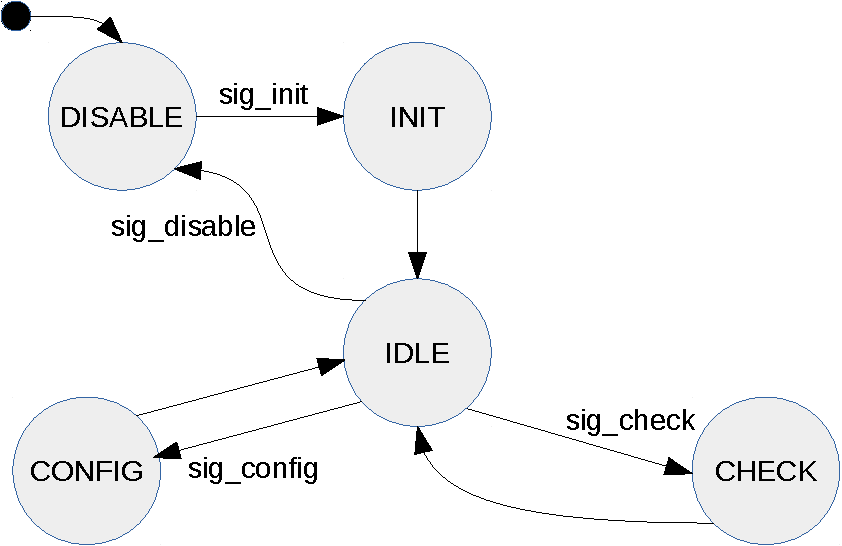
\includegraphics[width=\textwidth]{./Figures/MEF_generica.pdf}
	\caption[Diseño de MEF genérica para los módulos]{Diseño de máquina de estados finitos genérica para el control de la lógica de los módulos}
	\label{fig:mef_generica}
\end{figure}

\section{Módulo de almacenamiento}
\label{sec:almacenamiento}

El propósito del módulo de almacenamiento es proveer al sistema de una interfaz para operar con un medio de almacenamiento no volátil que permita guardar en forma permanente los datos registrados por el módulo de adquisición y eventualmente un log con información de \textit{debug}.

\subsection{Medio físico}
\label{subsec:mediofisico}

Se evaluaron distintas opciones de medios físicos.  En la tabla \ref{tab:medios} se recopilan las alternativas analizadas y se especifica un orden de magnitud para la capacidad de almacenamiento posible, el tipo de interfaz con el microcontrolador y el protocolo que debe implementarse en el \textit{firmware} para su utilización.

\vspace{10px}

\begin{table}[ht]
\centering
\caption{Alternativas de medios físicos evaluados.}
\label{tab:medios}
\begin{tabular}{lrcc}
\toprule
\multicolumn{1}{c}{\textbf{Medio físico}} & \multicolumn{1}{c}{\textbf{Capacidad}} & \textbf{Interfaz} & \textbf{Protocolo} \\ \midrule
USB Mass Storage Device                   & $\sim$10 Gb                            & USB 2.0           & USB                \\
Tarjeta de memoria microSD                & $\sim$10 Gb                            & Micro SD          & SSP                \\
Disco de estado sólido (SSD)              & $\sim$100 Gb                           & SATA III          & SATA               \\
Disco duro mecánico (HHD)                 & $\sim$1000 Gb                          & SATA III          & SATA               \\ \bottomrule
\end{tabular}
\end{table}

\vspace{10px}

Teniendo en cuenta criterios de costos y simplicidad de interacción con la CIAA-NXP, se decidió utilizar un lector de tarjetas microSD con comunicación sobre un puerto \textit{Synchronous Serial Port} (SSP).  Este protocolo es compatible con el protocolo SPI y utiliza un bus de 4 cables con las señales SCK, SSEL, MISO y MOSI.  Asimismo, el soporte seleccionado minimiza el consumo de energía respecto a las otras alternativas, lo cual lo hace deseable para la aplicación.

El lector de tarjetas utilizado se presenta en la figura \ref{fig:lector_sdCard}, donde puede verse esquemáticamente el diagrama de conexionado eléctrico entre la CIAA-NXP y el lector (figura \ref{fig:lector_conexionado}) y una vista superior del módulo de hardware (figura \ref{fig:lector_hardware}). Cabe notar que al haber un único dispositivo ``escalvo'' en el bus SSP, la señal de \textit{chip select} (CS) se conecta con GND, lo que implica que el dispositivo está permanente seleccionado.

\vspace{20px}

\renewcommand{\thesubfigure}{\alph{subfigure}}

\begin{figure}[h]
	\centering
	\begin{subfigure}{.4\textwidth}
		\centering
		\begin{tabular}{rll}
			\textbf{CIAA-NXP }&	& \textbf{Lector de tarjetas}\\
			+3.3V     & --\textgreater{} & +3.3V   \\
			GND       & --\textgreater{} & CS  \\
			SPI\_MOSI & --\textgreater{} & MOSI  \\
			SPI\_SCK  & --\textgreater{} & SCK \\
			SPI\_MISO & --\textgreater{} & MISO  \\
			GND       & --\textgreater{} & GND  \\
		\end{tabular}
		\caption{}
  		\label{fig:lector_conexionado}
	\end{subfigure}%
	\begin{subfigure}{.6\textwidth}
	\hspace{15px}
		\centering
		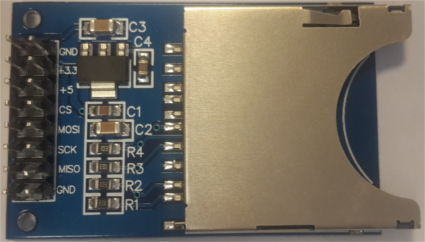
\includegraphics[height=3.3cm]{./Figures/sdCardReader.jpg}
		\caption{ }
		\label{fig:lector_hardware}
	\end{subfigure}
	\caption{(A) Diagrama de conexionado eléctrico y (B) Lector de tarjetas SD utilizado.}
	\label{fig:lector_sdCard}
\end{figure}

\vspace{10px}

Para la utilización del lector de tarjetas se hizo uso de la biblioteca FatFs, desarrollada por chaN \citep{fatFS}. FatFs es un módulo de sistema de archivos FAT/exFAT genérico para sistemas embebidos limitados en recursos. En la figura \ref{fig:chan} se esquematizan las interfaces de la biblioteca en una aplicación típica.

\begin{figure}[htpb]
	\centering
	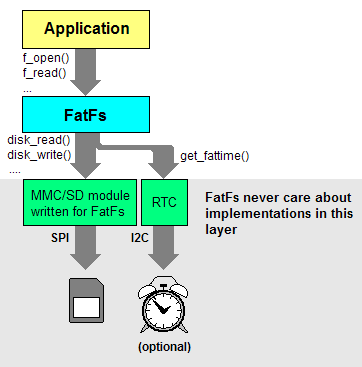
\includegraphics[width=.5\textwidth]{./Figures/chan.png}
	\caption[Diagrama de capas de fatFs]{Diagrama de capas con la ubicación de la biblioteca fatFs en el sistema y sus interfaces\protect\footnotemark.}
	\label{fig:chan}
\end{figure}

\footnotetext{Imagen tomada de \url{http://elm-chan.org/fsw/ff/doc/appnote.html}.}

El código está escrito en ANSI C y es \textit{software} libre bajo licencia estilo BSD \citep{BSD}.

\subsection{Máquina de Estados Finitos}
\label{subsec:MEFsdcard}

Se presenta el diagrama de estado de la MEF principal del módulo en la figura \ref{fig:mef_sdcard}, donde puede apreciase el punto de entrada con un circulo negro, los estado que puede tomar la máquina y las señales que provocan los cambios de estado. Se omiten del gráfico las salidas del sistema por simplicidad.

Debe notarse que al energizarse el sistema o luego de un \textit{reset}, el módulo se encuentra deshabilitado, con la MEF en el estado \texttt{DISABLE}, del cual sólo puede salir si se recibe una señal de inicialización.

Una vez inicializado, el módulo se encontrará la mayor parte del tiempo en el estado \texttt{IDLE} a la espera de un comando válido.

Cuando el módulo esté realizando alguna operación de lectura, escritura o actualización sobre la tarjeta SD, el estado del módulo tendrá el valor \texttt{PROCESSING} para indicarle al módulo de control que debe tener acceso a tiempo de CPU para poder completar las operaciones pendientes.

Todas las operación del módulo desde que es inicializado terminan incondicionalmente en el estado \texttt{IDLE}, en donde el valor de la variable que registra el estado del módulo cambia de \texttt{PROCESSING} a \texttt{READY}.

\begin{figure}[htpb]
	\centering
	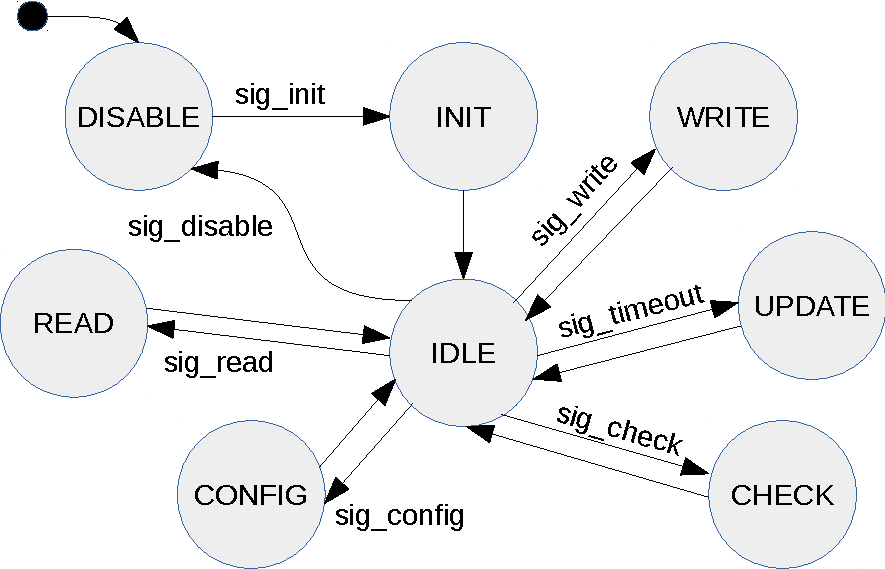
\includegraphics[width=\textwidth]{./Figures/MEF_sdCard_2.pdf}
	\caption[MEF principal del módulo de almacenamiento sdCard]{Máquina de estados finitos principal del módulo de almacenamiento.}
	\label{fig:mef_sdcard}
\end{figure}

%  Se indican las señales que puede recibir junto con las acciones más relevantes de cada estado. principal del módulo de almacenamiento

En la tabla \ref{tab:estadosAlmacenamiento} se describen los posibles estados de la MEF junto con las señales para alcanzarlos. Asimismo se explicitan las acciones y actividades más destacables que se realizan en cada uno de ellos.

% Please add the following required packages to your document preamble:
% \usepackage{graphicx}
\begin{table}[htpb]
\centering
\caption[Descripción de los estados de la MEF principal del módulo de almacenamiento.]{Descripción de los estados de la MEF principal del módulo de almacenamiento.}
\label{tab:estadosAlmacenamiento}
\resizebox{\textwidth}{!}{%
\begin{tabular}{lll}
\toprule
\multicolumn{1}{c}{\textbf{Estado}} & \multicolumn{1}{c}{\textbf{Señal para cambio}} & \multicolumn{1}{c}{\textbf{Acciones y actividades}} \\ \midrule
DISABLE & Reset o sig\_disable & \begin{tabular}[c]{@{}l@{}}Desinicializar el controlador SPI.\\ Desinicializar la bilioteca fatFS.\\ Desinicializar el módulo de almacenamiento.\\ Cambiar el estado del módulo de READY a DISABLE.\end{tabular} \\
 &  &  \\
INIT & sig\_init & \begin{tabular}[c]{@{}l@{}}Inicializar el controlador SPI.\\ Inicializar la bilioteca fatFS.\\ Inicializar el módulo de almacenamiento.\\ Cambiar el estado del módulo de DISABLE a READY.\end{tabular} \\
 &  &  \\
IDLE & transición incondicional & Cambiar estado del módulo de PROCESSING a READY. \\
 &  &  \\
CONFIG & sig\_config & Realizar cambios de configuración al módulo. \\
 &  &  \\
CHECK & sig\_check & Realizar autochequeo e informar al módulo de control \\
 &  &  \\
UPDATE & sig\_timeout & Ejecutar tarea periódica de actualización de la tarjeta SD. \\
 &  &  \\
WRITE & sig\_write & Obtener timestamp y escribir datos en la tarjeta SD. \\
 &  &  \\
READ & sig\_read & Leer datos en la tarjeta SD \\ \bottomrule
\end{tabular}%
}
\end{table}


\clearpage
\section{Módulo de adquisición}
\label{sec:adquisicion}

El propósito del módulo de adquisición es proveer al sistema de una interfaz para operar los distintos sensores que puedan conectarse a la estación.  Originalmente, se contempló el uso de uno o varios termómetros y un anemómetro para medir temperatura del agua y velocidad del viento en superficie, respectivamente. Adicionalmente, se contempla incorporar hidrofónos para registrar el nivel de ruido submarino, principal objetivo de la estación de medición.

Se mencionó en la sección \ref{sec:objetivosyalcances}, que los hidrófonos quedaron fuera del alcance del proyecto en esta etapa del desarrollo.  De igual manera, el control del anemómetro quedará fuera de la implementación ya que se optó por priorizar el requerimiento implícito de cumplir con la fecha de entrega.  Se retoma este punto en el capítulo \ref{Chapter5}, en la sección \ref{subsec:metasalcanzadas}, donde se discuten sus implicancias.

Sin pérdida de generalidad, la arquitectura de módulo adoptada puede utilizarse para incorporar los sensores no implementados, en una segunda iteración.

\subsection{Sensor de temperatura}
\label{subsec:1-wire}

%En la presente sección se presenta la implementación del control para el sensor de temperatura.

Se evaluaron distintas opciones de sensores de temperatura disponibles en el mercado local.  Se recopila en la tabla \ref{tab:temperatura} la información relevada para los sensores candidatos, donde se indican fabricante y modelo de cada dispositivo junto con las principales características de interés para la aplicación.

Cabe destacar que el rango de temperatura de todos los sensores analizados está limitado principalmente por el plástico que recubre los hilos conductores que lo conectan al microcontrolador, motivo por el cual todas las alternativas evaluadas poseen rangos equivalente.  Se utiliza en la tabla un código sencillo para indicar un orden de magnitud del costo relativo del sensor con \$ para costo bajo, \$\$ para costo medio y \$\$\$ para costo alto.

% Please add the following required packages to your document preamble:
% \usepackage{graphicx}
\begin{table}[htpb]
\centering
\caption{Alternativas de sensor de temperatura evaluadas.}
\label{tab:temperatura}
\resizebox{\textwidth}{!}{%
\begin{tabular}{ccccccc}
\toprule
\textbf{Fabricante} & \textbf{Sensor} & \textbf{Tipo} & \textbf{Precisión (\grados C)} & \textbf{Rango (\grados C)} & \textbf{Interfaz} & \textbf{Costo} \\
\midrule
Maxim Integrated    & DS18B20     & Termómetro digital & $\pm$ 0.5 & -55 a +125   & 1-wire & \$             \\
\multicolumn{1}{l}{} & \multicolumn{1}{l}{} & \multicolumn{1}{l}{} & \multicolumn{1}{l}{} & \multicolumn{1}{l}{} & \multicolumn{1}{l}{} & \multicolumn{1}{l}{} \\
Genérico            & IM120628010 & Termistor NTC & 1\% & -25 a +125   & 1-wire & \$             \\
\multicolumn{1}{l}{} & \multicolumn{1}{l}{} & \multicolumn{1}{l}{} & \multicolumn{1}{l}{} & \multicolumn{1}{l}{} & \multicolumn{1}{l}{} & \multicolumn{1}{l}{} \\
Texas Instruments         & LM35  & Integrated Circuit & $\pm$ 0.5 & -55 a +150   & \textit{Analog}         & \$   \\
\multicolumn{1}{l}{} & \multicolumn{1}{l}{} & \multicolumn{1}{l}{} & \multicolumn{1}{l}{} & \multicolumn{1}{l}{} & \multicolumn{1}{l}{} & \multicolumn{1}{l}{} \\
Altas Scientific    & PT-1000A    & \begin{tabular}[c]{@{}c@{}}RTD \\ (resistance\\ temperature\\ detector)\end{tabular} & $\pm$ (0.15 + 0.002*t)  & -55 a +125   & \textit{Analog}         & \$\$\$         \\
\bottomrule
\end{tabular}%
}
\end{table}

El sensor elegido es el termómetro digital DS18B20 del fabricante Maxim Integrated \citep{ds18b20}. Los motivos de la elección fueron principalmente la facilidad de uso en un entorno embebido de recursos limitados, la disponibilidad de documentación completa y detallada junto con numerosas notas de aplicación y el bajo costo del dispositivo.

En la figura \ref{fig:ds18b20_bloques} se puede apreciar un diagrama en bloques del sensor, en donde destaca la interfaz de 3 cables con una línea bidireccional de datos (DQ) y dos cables para la alimentación (GND y $V_{DD}$).

El sensor admite una configuración de alimentación ``parásita'', en la cual se energiza desde la línea de datos DQ, lo que habilita a prescindir de un cable a costa de mayores requerimientos para la temporización de las comunicaciones y la utilización de un transistor a modo de \textit{``strong pull-up''} (conectado el bus de datos directamente a $V_{DD}$).

\begin{figure}[htpb]
	\centering
	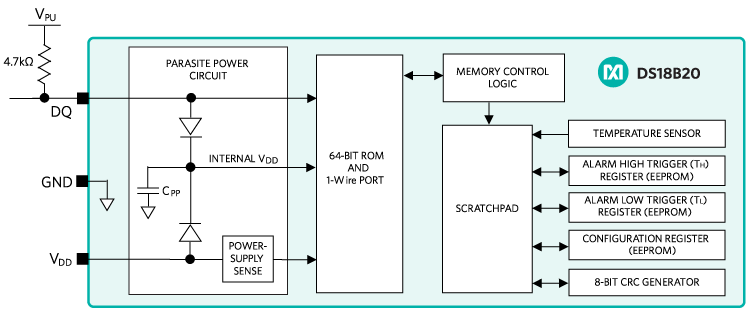
\includegraphics[width=.8\textwidth]{./Figures/ds18b20_bloques.png}
	\caption[Diagrama en bloques del sensor de temperatura DS18B20]{Diagrama en bloques del sensor de temperatura\protect\footnotemark.}
	\label{fig:ds18b20_bloques}
\end{figure}

\footnotetext{Imagen tomada de \url{https://www.maximintegrated.com/en/images/qv/2812.png}}

Cada sensor posee un código de identificación único de 64 bits que permite operar con múltiples sensores sobre un mismo bus de tipo 1-wire.  Mediante un algoritmo de descubrimiento se pueden identificar los sensores conectados a un mismo bus y controlarlos independientemente.

La capacidad para identificar cuántos sensores hay conectados en cada momento y poder interrogarlos individualmente se utilizó para incorporar una funcionalidad de autochequeo, en la cual el microcontrolador es capaz de detectar si un sensor ha dejado de funcionar correctamente.

Otras características destacables son la posibilidad de configurar la resolución entre 9 y 12 bits, el uso de CRC en las comunicaciones y la capacidad para definir umbrales de alarma para los valores de temperatura medidos.

Este sensor se comercializa con distintas longitudes de cable, dentro de un encapsulado metálico sumergible.  Para este trabajo se adquirieron dos sensores sumergibles con 5 metros de cable y 2 metros de cable, respectivamente.

Los dos sensores operan sobre una misma línea de datos con una resistencia de \textit{pull-up} de 2,2 K$\Omega$, como puede verse en el diagrama de conexionado eléctrico de la figura \ref{fig:ds18b20_conexionado}.  El encapsulado sumergible puede apreciarse en la figura \ref{fig:termometro}.

%\vspace{10px}

\begin{figure}[htpb]
	\centering
	\begin{subfigure}{.6\textwidth}
		\centering
		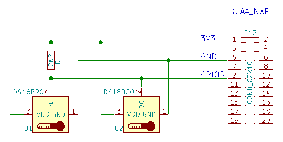
\includegraphics[height=3.7cm]{./Figures/ds18b20_conexionado.pdf}
		\caption{ Diagrama de conexionado eléctrico}
  		\label{fig:ds18b20_conexionado}
	\end{subfigure}%
	\begin{subfigure}{.4\textwidth}
		\centering
		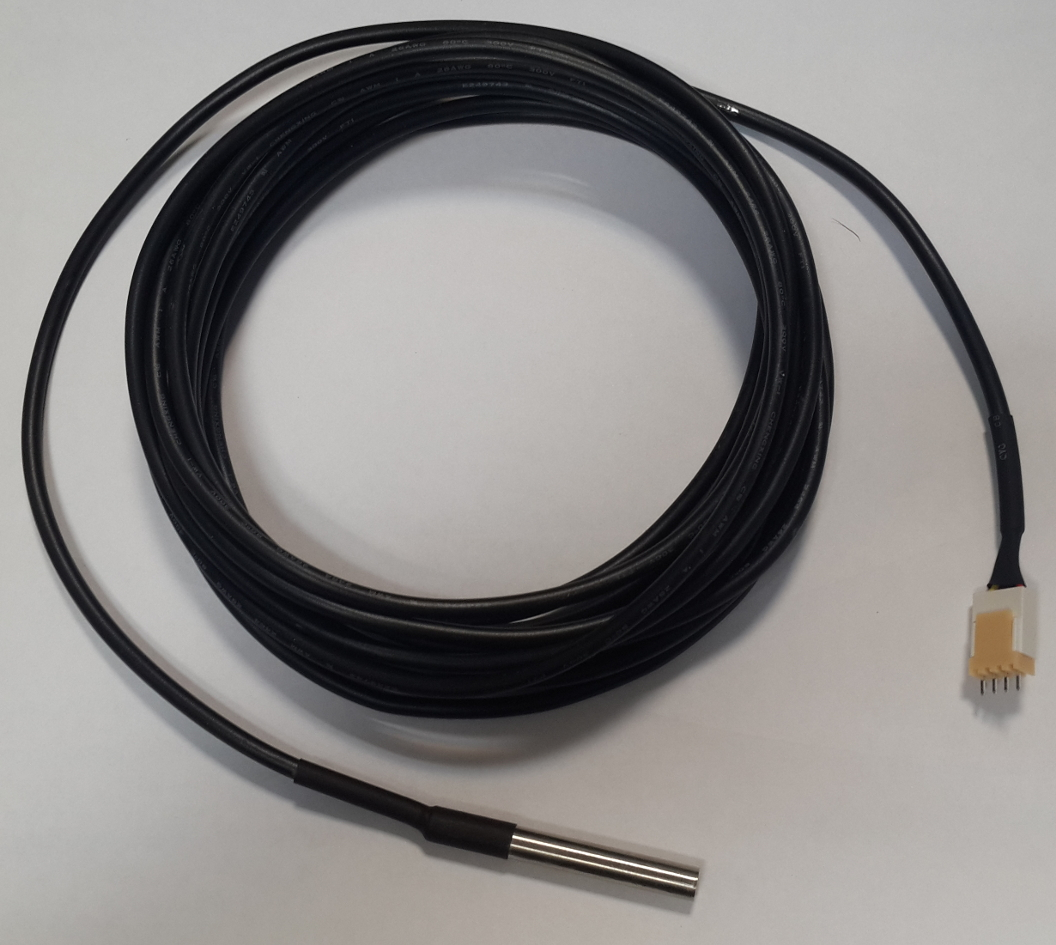
\includegraphics[height=3.7cm]{./Figures/ds18b20.jpg}
		\caption{ Sensor DS18B20}
		\label{fig:termometro}
	\end{subfigure}
	\caption{}
	\label{fig:ds18b20}
\end{figure}


Para el control de los dispositivos se adaptó una implementación de controlador de bus \textit{1-wire} para microcontroladores de la familia LPC1343, desarrollada en forma de biblioteca por James Harwood \citep{harwood}.  En esta biblioteca se hace uso de las técnicas de programación concurrente descriptas en la subsección \ref{subsec:protothreads}.

\subsection{Máquina de Estados Finitos}

En forma análoga a lo presentado en la subsección \ref{subsec:MEFsdcard}, se muestra aquí el diagrama de estado de la MEF principal del módulo en la figura \ref{fig:mef_adquisicion}, donde puede apreciase el punto de entrada con un circulo negro, los estado que puede tomar la máquina y las señales que provocan los cambios de estado. Se omiten del gráfico las salidas del sistema por simplicidad.

Igualmente, debe notarse que cuando el sistema es energizado o luego de un \textit{reset}, el módulo se encuentra deshabilitado, con la MEF en el estado \texttt{DISABLE}, del cual sólo puede salir si se recibe una señal de inicialización.

Una vez inicializado, el módulo se encontrará la mayor parte del tiempo en el estado \texttt{IDLE} a la espera de un comando válido.

Cuando el módulo esté realizando alguna operación de adquisición, configuración o autochequeo sobre los sensores conectados, el estado del módulo tendrá el valor \texttt{PROCESSING} para indicarle al módulo de control que debe tener acceso a tiempo de CPU para poder completar las operaciones pendientes.

Todas las operación del módulo desde que es inicializado terminan incondicionalmente en el estado \texttt{IDLE}, en donde el valor de la variable que registra el estado cambia de \texttt{PROCESSING} a \texttt{READY}.

\begin{figure}[htpb]
	\centering
	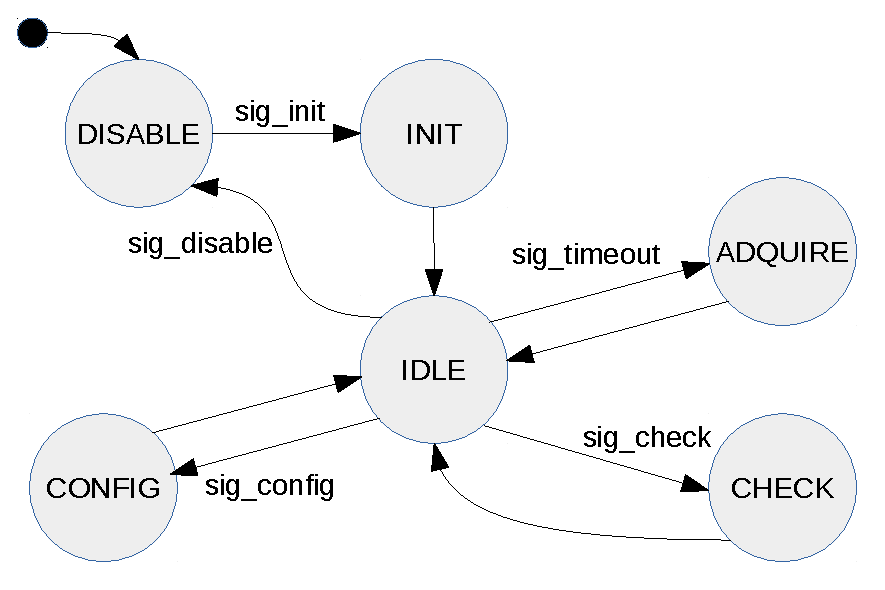
\includegraphics[width=\textwidth]{./Figures/MEF_adquisicion.pdf}
	\caption[MEF principal del módulo de adquisición de temperatura]{Máquina de estados finitos principal del módulo de adquisición de temperatura}
	\label{fig:mef_adquisicion}
\end{figure}

Las principales acciones y actividades de cada estado se describen en la tabla \ref{tab:estadosAdquisicion}.  Asimismo, se indican las señales válidas que puede recibir la MEF junto con las transiciones que éstas provocan.

% Please add the following required packages to your document preamble:
% \usepackage{graphicx}
\begin{table}[htpb]
\centering
\caption[Descripción de los estados de la MEF principal del módulo de adquisición.]{Descripción de los estados de la MEF principal del módulo de adquisición.  Se indican las señales que puede recibir junto con las acciones más relevantes de cada estado.}
\label{tab:estadosAdquisicion}
\resizebox{\textwidth}{!}{%
\begin{tabular}{lll}
\toprule
\multicolumn{1}{c}{\textbf{Estado}} & \multicolumn{1}{c}{\textbf{Señal para cambio}} & \multicolumn{1}{c}{\textbf{Acciones y actividades}} \\ \midrule
DISABLE & Reset o sig\_disable & \begin{tabular}[c]{@{}l@{}}Desinicializar el TIMER0.\\ Deshabilitar la interrupción TIMER0\_IRQn. \\ Desinicializar el GPIO 3[0].\\ Cambiar el estado del módulo de READY a DISABLE.\end{tabular} \\
 &  &  \\
INIT & sig\_init & \begin{tabular}[c]{@{}l@{}}Inicializar el TIMER0.\\ Habilitar la interrupción TIMER0\_IRQn.\\ Inicializar el GPIO3[0].\\ Cambiar el estado del módulo de DISABLE a READY.\end{tabular} \\
 &  &  \\
IDLE & transición incondicional & Cambiar estado del módulo de PROCESSING a READY. \\
 &  &  \\
CONFIG & sig\_config & Realizar cambios de configuración al módulo. \\
 &  &  \\
CHECK & sig\_check & Realizar autochequeo e informar al módulo de control \\
 &  &  \\
ADQUIRE & sig\_timeout & Ejecutar tarea periódica de adquisición de datos \\ \bottomrule
\end{tabular}%
}
\end{table}
%\subsection{Sensor de velocidad de viento}
%\label{subsec:anemometro}

\section{Módulo interfaz máquina-hombre}
\label{sec:HMI}

El propósito del módulo interfaz máquina-hombre (HMI, por sus siglas en inglés) es proveer al sistema de un medio de interacción con un operador humano. Las posibles interacciones se realizan a través de una interfaz de comandos interactiva y contempla operaciones de configuración y cambio de parámetros sobre los módulos y operaciones de mantenimiento y depuración del sistema.

La interfaz se implementa desde el microcontrolador sobre un puerto serie de tipo \textit{Universal Asynchronous Receiver-Transmitter} o UART a través de un conversor RS232/USB de la firma FTDI incorporado en la CIAA-NXP, hasta llegar finalmente a la PC del operador humano.

El código del módulo incluye directivas de compilación condicional que permiten cambiar la cantidad y el nivel de detalle de los mensajes que el sistema envía a través de la interfaz.  Esta opción debe definirse en tiempo de compilación y no puede ser modificada en tiempo de ejecución, es decir, una vez que el sistema esté en funcionamiento.

Mediante una directiva \texttt{DEFINE} para el precompilador se puede definir el símbolo \texttt{DEBUG\_ENABLE} en el archivo \texttt{board\_api.h}.   Si esta macro se encuentra definida, se habilitan funciones de depuración que envían mensajes a través de la UART como puede verse en el algorirmo \ref{lst:debug}.

%\begin{verbatim}
%  #define DEBUG_ENABLE
%\end{verbatim}

Adicionalmente, si se define la MACRO \texttt{DEBUG\_SEMIHOSTING} se pueden utilizar los recursos de entrada/salida de la PC host que esté depurando el sistema embebido.

Si la MACRO \texttt{DEBUG\_ENABLE} no es definida, las funciones no se incluyen en el código, ahorrando recursos al sistema.

\vspace{10px}

\begin{lstlisting}[caption={Macros para habilitar/deshabilitar mensajes de depuración del código.},label={lst:debug}]
#if defined(DEBUG_ENABLE)

  #if defined(DEBUG_SEMIHOSTING)

    #define DEBUGINIT()
    #define DEBUGOUT(...) printf(__VA_ARGS__)
    #define DEBUGSTR(str) printf(str)
    #define DEBUGIN() (int) EOF

  #else

    #define DEBUGINIT() Board_Debug_Init()
    #define DEBUGOUT(...) printf(__VA_ARGS__)
    #define DEBUGSTR(str) Board_UARTPutSTR(str)
    #define DEBUGIN() Board_UARTGetChar()

  #endif /* defined(DEBUG_SEMIHOSTING) */

#else

  #define DEBUGINIT()
  #define DEBUGOUT(...)
  #define DEBUGSTR(str)
  #define DEBUGIN() (int) EOF

#endif /* defined(DEBUG_ENABLE) */
\end{lstlisting}

Para acceder a la interfaz se debe utilizar una terminal serie tipo \texttt{screen} \citep{screen} en configuración 8N1 a 115200 baudios.

Existen emuladores de terminales serie como \textit{cutecom}, de gran difusión, que presentan el inconveniente de no implementar funciones de control definidas en los estándares ANSI X3.64 (ISO 6429) e ISO 2022 por lo que la visualización de la interfaz en estas consolas puede ser defectuosa y no se recomienda su uso.


\subsection{Interfaz}
\label{subsec:interfaz}

El propósito de la interfaz desarrollada es servir como prueba de concepto e incluye un mínimo de funcionalidad para cumplir los requerimientos relacionados a la controlabilidad de la estación, principalmente en lo referido al período de muestreo de los sensores del módulo de adquisición.

Cabe destacar que el valor de esta interfaz no está en su estética ni en su facilidad de uso, sino en la arquitectura subyacente que permite obtener información del sistema y operar sobre sus distintos componentes.

Una primera versión de la interfaz operativa se presenta en la figura \ref{fig:interfaz_main}, donde pueden apreciarse cuatro zonas funcionales identificadas con recuadros de color rojo, a saber: encabezado, menú de opciones, línea de comandos y barra de estado.

\begin{figure}[htpb]
	\centering
	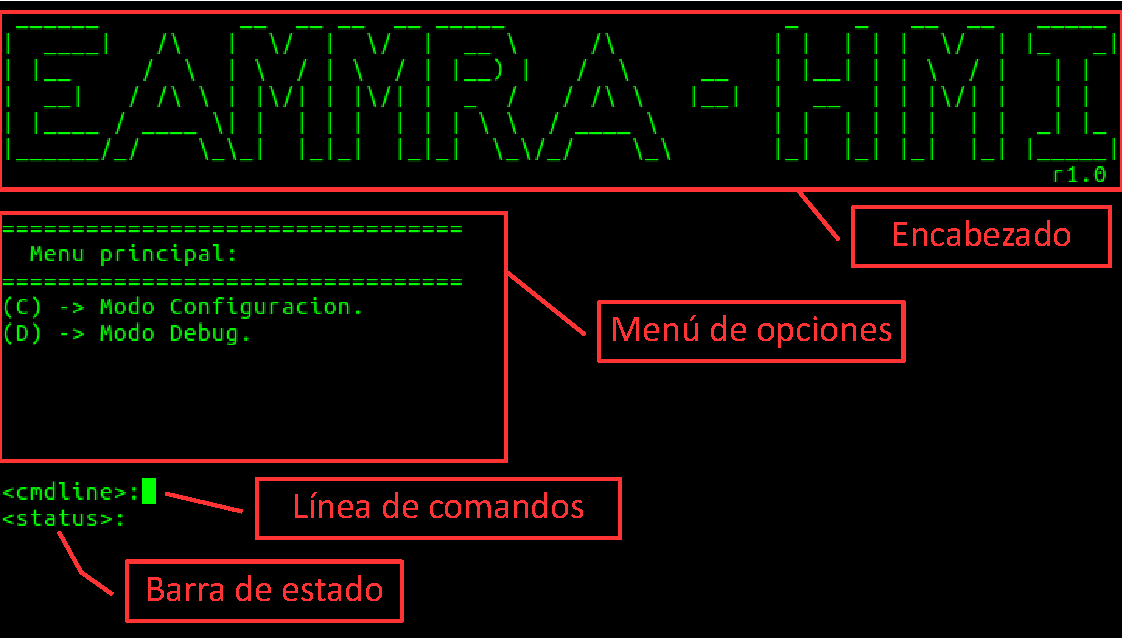
\includegraphics[width=\textwidth]{./Figures/interfaz_detalles.pdf}
	\caption[]{Vista de la pantalla principal de la interfaz. Se destacan con recuadros rojos cuatro secciones dentro de la pantalla: encabezado, menú de opciones, línea de comandos y barra de estado.}
	\label{fig:interfaz_main}
\end{figure}

En el encabezado puede observarse el nombre de la estación EAMMRA, por las siglas de ``Estación Autónoma Marítima de Medición de Ruido Ambiente'' junto en una identificación del número de revisión de la interfaz, en el caso de la figura \ref{fig:interfaz_main}, r1.0.

En la zona asociada al menú de opciones se presentan los comandos que puede introducir el operador. En cada pantalla, las opciones que se muestran cambian según el contexto.

Se realiza un eco de los comandos ingresados, que aparecen en la línea de comandos para confirmación del usuario. Asimismo, si se ingresa un caracter que no sea parte de las opciones disponibles, el sistema lo informa a continuación del eco con el mensaje `` no es un comando valido.''

Los diferentes módulos pueden enviar mensajes para el usuario que aparecerán en la sección indicada como barra de estado.  De igual manera, cuando el sistema requiera confirmación por parte del usuario, se exhibirá un mensaje para tal fin en esta sección.

Desde el menú principal se puede acceder al modo configuración para interactuar directamente con los módulos del sistema.  Se presenta la pantalla principal de este modo en la figura \ref{fig:interfaz_config}.  Para acceder a las opciones de un módulo en particular se debe ingresar el número asociado a éste en el menú de opciones.  A excepción de la pantalla principal, todas las pantallas cuentan con una opción (X) para volver al menú anterior.

\begin{figure}[htpb]
	\centering
	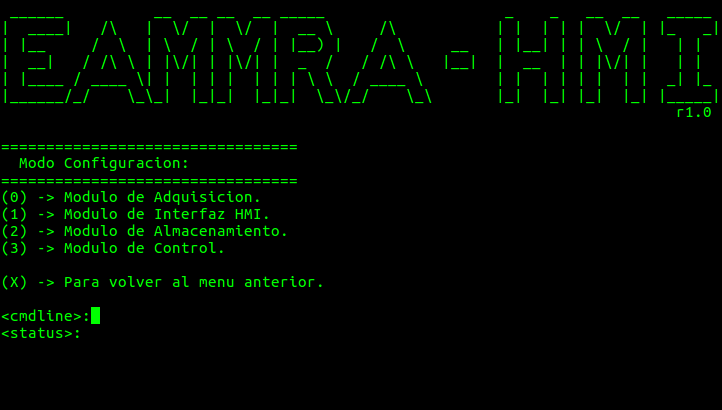
\includegraphics[width=\textwidth]{./Figures/interfaz_config.png}
	\caption[]{Vista de la pantalla principal del modo configuración de la interfaz máquina-hombre.}
	\label{fig:interfaz_config}
\end{figure}

Sin pérdida de generalidad, ya que todos los módulos comparten las mismas opciones, se presenta en la figura \ref{fig:interfaz_config_detalle} una vista de detalle de la pantalla de configuración del módulo de adquisición, también llamado módulo 1-WIRE por el tipo de sensor que controla. Se puede observar la opción de configuración elegida en la línea de comandos y el pedido de confirmación en la barra de estado.

Se contempla diferenciar a futuro las opciones de cada módulo acorde se agregue funcionalidad a los mismos. Las opciones actualmente disponibles son las siguientes:

\begin{itemize}
  \item \texttt{(D)} Habilitar / Deshabilitar: permite intercambiar el estado del módulo entre \texttt{READY} y \texttt{DISABLED}.  Para tal fin, si el módulo se encuentra en estado \texttt{READY}, se le envía una señal sig\_disable.  En caso que se encuentre en estado \texttt{DISABLED} se le envía una señal sig\_init.  Antes de enviar la señal correspondiente se informa al usuario el estado actual del módulo y se pide que confirme o cancele la operación mediante el ingreso de \texttt{`s'} o \texttt{`n'}, respectivamente.
  \item \texttt{(I)} Info del módulo: muestra el estado actual del módulo en la barra de estado.  Las respuestas posibles son \texttt{READY}, \texttt{PROCESSING} y \texttt{DISABLED}
  \item \texttt{(C)} Configurar: permite cambiar la configuración del módulo.  En esta etapa del desarrollo se implementó únicamente la posibilidad de cambiar el tiempo con que se ejecuta la tarea periódica, si la hubiera.
  \item \texttt{(A)} Autocomprobación: permite realizar una comprobación interna de funcionamiento mediante el envío de una señal sig\_check al módulo. En esta etapa del desarrollo la funcionalidad está implementada con una función \textit{mock} que devuelve un mensaje en la barra de estado.
  \item \texttt{(X)} para volver al menú anterior: cambia el menú a la pantalla principal del modo configuración.
\end{itemize}

\begin{figure}[htpb]
	\centering
	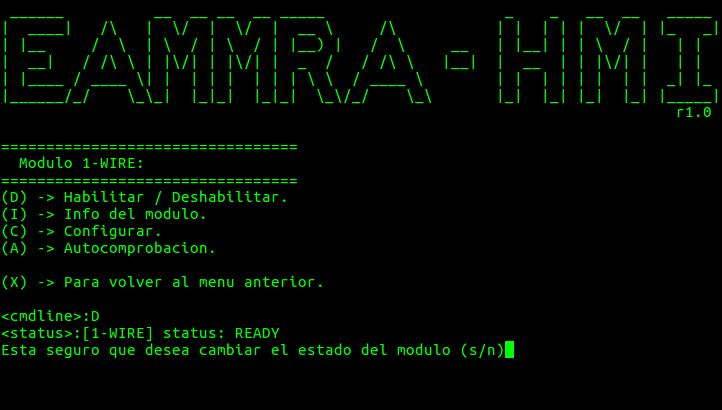
\includegraphics[width=\textwidth]{./Figures/interfaz_config_detalle.png}
	\caption[Pantalla de configuración del módulo de adquisición.]{Pantalla de configuración del módulo de adquisición con una operación de deshabilitación en curso.}
	\label{fig:interfaz_config_detalle}
\end{figure}

Asimismo, desde el menú principal se puede acceder a un modo \textit{debug} con opciones de depuración y mantenimiento como puede observarse en la figura \ref{fig:interfaz_debug}.

\begin{figure}[htpb]
	\centering
	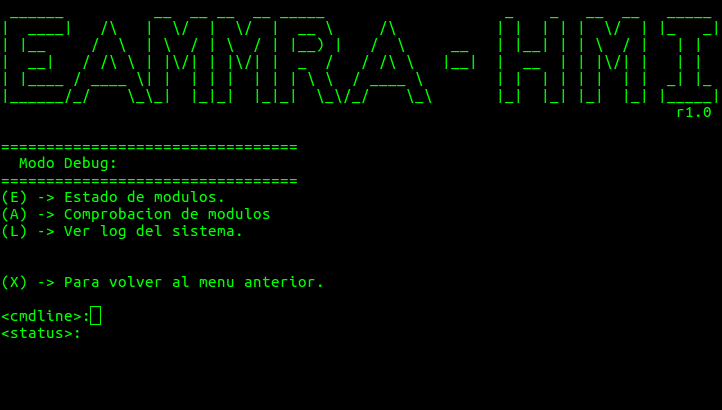
\includegraphics[width=\textwidth]{./Figures/interfaz_debug.png}
	\caption{Vista de la pantalla principal del modo debug de la interfaz máquina-hombre.}
	\label{fig:interfaz_debug}
\end{figure}

Las opciones para este modo son:

\begin{itemize}
  \item \texttt{(E)} Estado de módulos: muestra el estado actual de todos los módulo del sistema en la barra de estado.
  \item \texttt{(A)} Comprobación: permite realizar una comprobación interna de funcionamiento a todos los módulos. En esta etapa del desarrollo la funcionalidad está implementada con una función \textit{mock} que devuelve un mensaje en la barra de estado y registra los resultados en el log del sistema.
  \item \texttt{(L)} Ver log del sistema: permite realizar un \textit{dump} del log del sistema en la consola.  Esto significa que se imprime en la terminal serie todo el contenido del archivo de log ubicado en la tarjeta de memoria microSD. Presionando cualquier tecla se limpia la pantalla y se vuelve al menú principal del modo \textit{debug}.
  \item \texttt{(X)} para volver al menú anterior: cambia el menú a la plantalla principal del modo \textit{debug}.
\end{itemize}

En la tabla \ref{tab:interfaz_config}, se recopilan los comandos que se pueden ingresar por la interfaz en el modo configuración junto con una descripción de la funcionalidad que activa en el sistema.  Asimismo, se explicita si la función se encuentran implementada o maquetada.

\begin{table}[htpb]
\centering
\caption{Opciones disponibles en el modo configuración de la interfaz.  Se indica el comando para seleccionar la opción y si ésta se encuentra implementada o maquetada.}
\label{tab:interfaz_config}
%\resizebox{\textwidth}{!}{%
\begin{tabular}{ccccc}
\toprule
\textbf{\textbf{Opción}} & \textbf{Descripción} & \textbf{Implementada} & \textbf{Maquetada} \\ \midrule
D & \begin{tabular}[c]{@{}c@{}}Habilitar / Deshabilitar el módulo.\\ Se informa el estado actual\\ Se pide confirmación del usuario\end{tabular} & X &  \\
\multicolumn{1}{l}{} & \multicolumn{1}{l}{} & \multicolumn{1}{l}{} & \multicolumn{1}{l}{} \\
I & Informa el estado del módulo. & X &  \\
\multicolumn{1}{l}{} & \multicolumn{1}{l}{} & \multicolumn{1}{l}{} & \multicolumn{1}{l}{} \\
C & \begin{tabular}[c]{@{}c@{}}Configurar el módulo\\ Permite cambiar el valor de\\ period dentro de la estructura\\ de control del módulo\end{tabular} & X &  \\
\multicolumn{1}{l}{} & \multicolumn{1}{l}{} & \multicolumn{1}{l}{} & \multicolumn{1}{l}{} \\
A & \begin{tabular}[c]{@{}c@{}}Autocomprobación del módulo.\\ Informa en la barra de estado\\ el resultado de la verificación.\end{tabular} &  & X \\ \bottomrule
\end{tabular}%
%}
\end{table}

En forma análoga, se presenta en la tabla \ref{tab:interfaz_debug}, una recopilación de los comandos que se pueden ingresar en el modo debug junto con una descripción de la misma.  Asimismo, se explicita si la función se encuentran implementada o maquetada.

\begin{table}[htpb]
\centering
\caption{Opciones disponibles en el modo debug de la interfaz.  Se indica el comando para seleccionar la opción y si ésta se encuentra implementada o maquetada.}
\label{tab:interfaz_debug}
%\resizebox{\textwidth}{!}{%
\begin{tabular}{cccc}
\toprule
\textbf{Opción} & \textbf{Descripción} & \textbf{Implementada} & \textbf{Maquetada} \\ \midrule
E & \begin{tabular}[c]{@{}c@{}}Informa el estado actual\\ de todos los módulos \\ en la barra de estado\end{tabular} & X &  \\
\multicolumn{1}{l}{} & \multicolumn{1}{l}{} & \multicolumn{1}{l}{} & \multicolumn{1}{l}{} \\
A & \begin{tabular}[c]{@{}c@{}}Autocomprobación\\ de todos los módulos.\\ Se registra el resultado\\ en el log del sistema\end{tabular} &  & X \\
\multicolumn{1}{l}{} & \multicolumn{1}{l}{} & \multicolumn{1}{l}{} & \multicolumn{1}{l}{} \\
L & \begin{tabular}[c]{@{}c@{}}Listar el contenido del \\ log del sistema.\\ Se limpia presionando\\ cualquier tecla\end{tabular} & X & \\
\bottomrule
\end{tabular}
%}
\end{table}

En los módulos que tiene funciones maquetadas se reemplazó la llamada a la función que debería realizar la implementación por el envío de un mensaje generado en el propio módulo hacia la interfaz HMI.  De esta manera se puede comprobar el correcto funcionamiento de la interfaz y el circuito de  comunicación entre módulos, es decir, que:

\begin{itemize}
	\item el comando es correctamente recibido por la interfaz,
	\item la interfaz envía correctamente una señal al módulo correspondiente,
	\item el módulo correspondiente recibe la señal y contesta con un mensaje que se visualiza en la barra de estado de la interfaz.
\end{itemize}

Se contempla incluir en versiones futuras, además de cambios estilísticos, la implementación completa de las funcionalidades que en la presente versión se encuentran maquetadas.  Si bien estás y otras características son deseable para la usabilidad de la interfaz y la operación de la estación, no formaban parte de los requerimientos enumerados en la sección \ref{sec:requerimientos}.



\subsection{Máquina de estados finitos}

El diagrama de estado de la MEF principal del módulo puede apreciarse en la figura \ref{fig:mef_HMI}, donde se observa el punto de entrada con un circulo negro, los estados que puede tomar la máquina y las señales que provocan los cambios de estado. Se omiten del gráfico las salidas del sistema por simplicidad.

Igualmente, debe notarse que cuando el sistema es energizado o luego de un \textit{reset}, el módulo se encuentra deshabilitado, con la MEF en el estado \texttt{DISABLE}, del cual sólo puede salir si se recibe una señal de inicialización.

Una vez inicializado, el módulo se encontrará la mayor parte del tiempo en el estado \texttt{IDLE} a la espera de un comando válido para procesar.

Cuando el módulo esté realizando alguna operación de procesamiento de comandos recibidos por el usuario, configuración o autochequeo, el estado en la del módulo tendrá el valor \texttt{PROCESSING} para indicarle al módulo de control que debe tener acceso a tiempo de CPU para poder completar las operaciones pendientes.

Todas las operación del módulo desde que es inicializado terminan incondicionalmente en el estado \texttt{IDLE}, en donde el valor de la variable que registra el estado cambia de \texttt{PROCESSING} a \texttt{READY}.

\begin{figure}[htpb]
	\centering
	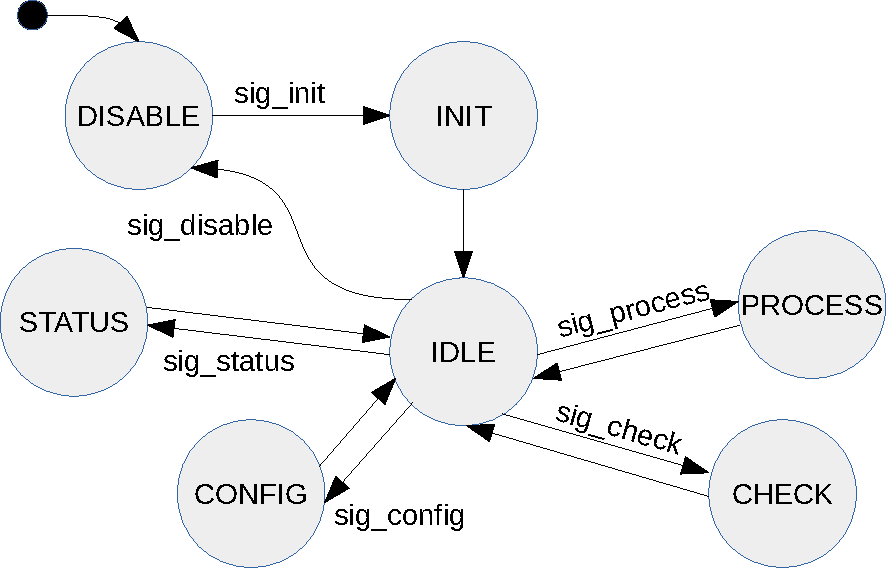
\includegraphics[width=\textwidth]{./Figures/MEF_HMI_2.pdf}
	\caption[MEF principal del módulo de HMI]{Máquina de estados finitos principal del módulo de interfaz máquina-hombre}
	\label{fig:mef_HMI}
\end{figure}

Se describen las principales acciones y actividades de cada estado en la tabla \ref{tab:estadosHMI}.  Asimismo, se indican las señales válidas que puede recibir la MEF junto con las transiciones que éstas provocan.


% Please add the following required packages to your document preamble:
% \usepackage{graphicx}
\begin{table}[htpb]
\centering
\caption[Descripción de los estados de la MEF principal del módulo HMI.]{Descripción de los estados de la MEF principal del módulo de interfaz máquina-hombre (HMI).  Se indican las señales que puede recibir junto con las acciones más relevantes de cada estado.}
\label{tab:estadosHMI}
\resizebox{\textwidth}{!}{%
\begin{tabular}{lll}
\toprule
\multicolumn{1}{c}{\textbf{Estado}} & \multicolumn{1}{c}{\textbf{Señal para cambio}} & \multicolumn{1}{c}{\textbf{Acciones y actividades}} \\ \midrule
DISABLE & Reset o sig\_disable & \begin{tabular}[c]{@{}l@{}}Desinicializar la UART.\\ Deshabilitar la interrupción de la UART. \\ Deshabilitar la transmisión de la UART\\ Cambiar el estado del módulo de READY a DISABLE.\end{tabular} \\
 &  &  \\
INIT & sig\_init & \begin{tabular}[c]{@{}l@{}}Inicializar la UART.\\ Habilitar la interrupción de la UART.\\ Habilitar la transmisión de la UART.\\ Cambiar el estado del módulo de DISABLE a READY.\end{tabular} \\
 &  &  \\
IDLE & transición incondicional & Cambiar estado del módulo de PROCESSING a READY. \\
 &  &  \\
CONFIG & sig\_config & Realizar cambios de configuración al módulo. \\
 &  &  \\
CHECK & sig\_check & Realizar autochequeo e informar al módulo de control \\
 &  &  \\
PROCESS & sig\_process & Procesar los comandos recibidos \\
 &  &  \\
STATUS & sig\_status & Enviar información de un módulo al usuario \\ \bottomrule
\end{tabular}%
}
\end{table}

\clearpage

\section{Módulo de control}
\label{sec:control}

El propósito del módulo de control es implementar un \textit{framework} o marco de trabajo para el funcionamiento de los demás módulos del sistemas.  En este sentido, provee los mecanismos de \textit{scheduling} para planificar la ejecución de las tareas del sistema y un \textit{dispatcher} para ejecutarlas.

Asimismo, se incluyen métodos para temporizar regularmente la ejecución de los módulos que requieran tareas periódicas mediante el uso de una base de tiempo con el \textit{sysTick timer} del microcontrolador.

Asimismo, este módulo implementa los mecanismos de comunicación entre procesadores descriptos en la subsección \ref{subsec:IPC} con algunas modificaciones.

En primer lugar se definieron dos colas de mensajes idénticas, una para cada procesador, como puede verse en el algoritmo \ref{lst:ipc_queue}.  Cada cola permite alojar una cantidad \texttt{IPCEX\_QUEUE\_SZ} de mensajes definida mediante una macro con valor numérico igual a 64.

\vspace{10px}

\begin{lstlisting}[caption={Definición de dos colas de eventos, una para cada procesador.},label={lst:ipc_queue}]
	/* Message QUEUE used by IPC library to exchange message between cores */
	static ipcex_msg_t ipcex_coreM4[IPCEX_QUEUE_SZ];
	static ipcex_msg_t ipcex_coreM0[IPCEX_QUEUE_SZ];
\end{lstlisting}


En segundo lugar, se permitió que los procesadores puedan escribir indistintamente en ambas colas, con el resguardo de activar la interrupción cruzada únicamente cuando el mensaje a encolar fuera para el otro procesador. Esta modificación es sencilla de implementar ya que la información del procesador de destino está contenida en el mismo mensaje.

De esta manera se proveyó un mecanismo de comunicación entre módulos definidos en un mismo procesador.  Asimismo, esto otorgó mayor flexibilidad al sistema en su conjunto, ya que a partir de esta modificación, el código de un módulo pueden incluirse en ambos procesadores y mediante una macro, elegir desde qué procesador se va a ejecutar, sin otras modificaciones en el resto del código.

Por otra parte, se modificó el tipo de dato \texttt{ipcex\_t} para contener, en lugar de dos campos de datos \texttt{uint32\_t}, un campo tipo signal\_t y otro tipo (void *) para el pasaje de parámetros genéricos, como puede verse en el algoritmo \ref{lst:msg_t}.

\vspace{10px}
\begin{lstlisting}[caption={Definición nuevo tipo de dato ipcex\_msg\_t para intercambio de mensajes.},label={lst:msg_t}]
	typedef struct __ipcex_msg {
	struct {
		cpuID_t cpu;
		moduleID_t pid;
	} id;
	signal_t signal;
	void *   param;
} ipcex_msg_t;
\end{lstlisting}

El tipo de dato \texttt{signal\_t} es una redefinición de una enumeración que contiene a todas las señales que es posible enviar a los módulos.  Su definición se puede apreciar en el algoritmo \ref{lst:signal_t}. Se define una última señal sig\_invalid para control de errores.

%\vspace{10px}
\begin{lstlisting}[caption={Definición nuevo tipo de dato signal\_t para el envío de señales a los módulos.},label={lst:signal_t}]
typedef enum {
	sig_disable,
	sig_init,
	sig_config,
	sig_check,
	sig_timeout,
	sig_process,
	sig_status,
	sig_adquire,
	sig_write,
	sig_read,
	sig_invalid
} signal_t;
\end{lstlisting}

Se obtiene acceso para controlar los distintos módulos que componen el sistema mediante el registro de un puntero a la estructura de control tipo \texttt{module\_t} de cada módulo, en un vector definido para tal fin.  Dicho vector se indexa mediante un índice tipo \texttt{moduleID\_t} cuya definición puede observarse en el algoritmo \ref{lst:moduleID_t}.  Se define un último índice \texttt{INVALID\_MODULE} para control de errores.

%\vspace{10px}
\begin{lstlisting}[caption={Definición nuevo tipo de dato moduleID\_t para indexar el control de los módulos.},label={lst:moduleID_t}]
typedef enum {
	ONEWIRE,
	HMI,
	SDCARD,
	CONTROL,
	INVALID_MODULE
} moduleID_t;
\end{lstlisting}

Las distintas estructuras de control son variables privadas definidas en archivos propios de cada módulo.  Para acceder a la direción de memoria que las contiene, cada módulo ofrece una interfaz \texttt{X\_get\_module\_pointer()} que devuelve por valor un puntero a \texttt{module\_t}. La \texttt{`X'} debe reemplazarse por el nombre del módulo correspondiente.  Se ejemplifica su uso en el algoritmo \ref{lst:register}.

%\vspace{10px}%
\begin{lstlisting}[caption={Función para registrar los módulos del sistema.},label={lst:register}]
void FR_register_all_modules(void){
	modules[ONEWIRE]  = ow_get_module_pointer();
	modules[HMI]      = hmi_get_module_pointer();
	modules[SDCARD]   = sd_get_module_pointer();
	modules[CONTROL]  = fr_get_module_pointer();
};
\end{lstlisting}

En el algoritmo \ref{lst:dispatcher} se presenta la función para despachar tareas y mensajes.  Se puede observar cómo primero se recorren los módulos en busca del \textit{flag} \texttt{runme} para ejecutar el manejador de eventos que tenga procesamiento pendiente. Se utiliza un mensaje especial vacio para este caso. Asimismo, se saca un mensaje de la cola si lo hubiere y se lo despacha al manejador de eventos correspondiente.

\vspace{10px}
\begin{lstlisting}[caption={Función para despachar tareas y mensajes.},label={lst:dispatcher}]
bool_t FR_dispatch_tasks(void){

	moduleID_t moduleID;
	ipcex_msg_t msg;
	bool_t goToSleep;

	for(moduleID=0;moduleID<INVALID_MODULE;moduleID++){
		if(modules[moduleID]->runme == TRUE)
			(*modules[moduleID]->eventHandler)(&msg_null);
	}

	if (IPC_tryPopMsg(&msg) == QUEUE_VALID) {
		if(msg.id.pid < INVALID_MODULE) {
			moduleID = msg.id.pid;
			if(modules[moduleID]->status == DISABLED &&
					msg.signal == sig_init)
				(*modules[moduleID]->eventHandler)(&msg);

			else if(modules[moduleID]->status == READY)
				(*modules[moduleID]->eventHandler)(&msg);

			else
				IPC_tryPushMsg(msg.id.cpu, &msg);
		}
		else
			DEBUGSTR("Error! msg.id.pid unknown\r\n");
	}

	goToSleep = TRUE;
	// Is there any module with processing pending?
	for(moduleID=0; moduleID<INVALID_MODULE; moduleID++) {
		if(modules[moduleID]->runme == TRUE)
			goToSleep = FALSE;
	}
	// Are there still messages in the queue?
	if ( IPC_msgPending(CPUID_CURR) != 0)
		goToSleep = FALSE;

	return goToSleep;
};
\end{lstlisting}

Para el despacho de eventos se toman los recaudos de observar que se haya sacado un mensaje válido de la cola y que el módulo destinatario del mensaje esté correctamente identificado.  A continuación, se consulta el estado del módulo.  Si el módulo está deshabilitado y el mensaje contiene una señal sig\_init se despacha el mensaje al módulo. Si el módulo se encuentra habilitado, se consulta si se encuentra en condiciones de recibir el mensaje (estado \texttt{READY}) en cuyo caso se despacha el mensaje al módulo.  En caso contrario, si el módulo se encuentre habilitado pero en estado \texttt{PROCESSING}, el mensaje se vuelve a introducir en la cola a la espera que el módulo termine el procesamiento pendiente.

Finalmente, se observa si quedan módulos con procesamiento pendiente y si hay mensajes en la cola sin atender.  Si alguna de estas condiciones resulta verdadera se deshabilita el \textit{flag} \texttt{goToSpleep} que se utiliza en el loop principal para saber si se debe poner el procesador en modo bajo consumo hasta que se produzca una interrupción.

En el algoritmo \ref{lst:main} se puede apreciar la estructura de \textit{super loop} del punto de entrada al código luego de la secuencia de \textit{startup}.  Aquí se realizan las inicializaciones generales que no sean propias de los módulos, se registran los punteros a las estructuras de control y se envía una señal de inicialización a todos los módulos correctamente registrados.  En el \textit{loop} principal se utiliza la macro \texttt{\_\_WFI()} para poner el procesdor en modo bajo consumo hasta la siguiente interrupción según el estado del \textit{flag} \texttt{goToSpleep} como ya fuera mencionado.

\vspace{10px}%
\begin{lstlisting}[caption={Función principal main().},label={lst:main}]
int main(void)
{
   bool_t goToSleep = FALSE;

   prvSetupHardware();
   FR_register_all_modules();
   FR_broadcast_signal(sig_init);

   while(TRUE) {  // the main loop

      goToSleep = FR_dispatch_tasks();

      if (goToSleep == TRUE)
         __WFI();
   }
   return 0;
}
\end{lstlisting}

Existe únicamente tres fuentes de interrupción posibles que pueden sacar al procesador del estado de bajo consumo, a saber:

\begin{itemize}
	\item Interrupción del sysTick Timer que se usa como base de tiempo en ms.
	\item Interrupción de la UART cuando se recibe un comando para la interfaz con el usuario.
	\item Interrupción del otro procesador para indicar que ha enviado un mensaje que requiere procesamiento.
\end{itemize}

En las rutinas de servicio de cada una de estas interrupciones se encolan los mensejes correspondientes que serán debidamente atendidos en la siguiente ejecución del despachador de eventos.

En en este módulo se implementa el control del perfil de consumo de energía del sistema, mediante lo cual se da cumplimiento al requerimiento  2.4.

Se definieron dos perfil de consumo distintos con las siguientes características:

\begin{itemize}
	\item Perfil 1: optimizado para \textit{performance}
	\begin{itemize}
		\item Todos los módulos habilitados
		\item Interrupción del sysTick Timer cada 1 ms
		\item Las adquisiciones de temperatura y su escritura en la microSD cada 1 segundo.
	\end{itemize}
	\item Perfil 2: optimizado para \textit{consumo}
	\begin{itemize}
		\item Módulo HMI deshabilitado
		\item Interrupción del sysTick Timer cada 10 ms
		\item Las adquisiciones de temperatura y su escritura en la microSD cada 10 segundo.
	\end{itemize}
\end{itemize}

El sistema se inicia con la configuración del perfil 1 de consumo eléctrico y pude pasar al perfil 2 si el usuario envía una señal de configuración para tal fin a través de la interfaz HMI. A los fines de esta etapa del desarrollo, una vez en el perfil 2, sólo es posible volver al perfil 1 reseteando el microcontrolador, ya que la interfaz HMI dejará de estar disponible.  Se contempla a futuro la posibilidad de intercalar ciclos de trabajo con los distintos perfiles según sea conveniente.

Por último, se menciona cuál fue la estrategia utilizada para asignar la ejecución de los módulos a los procesadores de la CIAA-NXP e integrar el sistema.  Se descarga el mismo \textit{firmware} a los  procesadores cortex-M0 y cortex-M4 con todas las funcionalidades del sistema.  Mediante un campo en la estructura de control de los módulos, \texttt{CPUID\_T coreID}, se puede cambiar el procesador que ejecuta el módulo, tomando el recaudo de deshabilitar previamente el módulo en el procesador que lo estuviera ejecutando al momento del cambio.

La configuración inicial adoptada se puede apreciar en la tabla \ref{tab:modulos}.

\begin{table}[ht]
\centering
\caption{Asignación de módulos a los procesadores}
\label{tab:modulos}
\begin{tabular}{lcccc}
\toprule
\textbf{Procesador} & \textbf{Control} & \textbf{sdCard} & \textbf{Adquisición} & \textbf{HMI} \\ \midrule
Cortex-M0			&                  &                 &                      & X            \\
Cortex-M4   		& X                & X               & X                    &              \\
\bottomrule
\end{tabular}
\end{table}

De esta forma, el procesador cortex-M0 permanecerá en modo bajo consumo la mayor parte del tiempo y sólo se activará cuando se produzca una interrupción.  Las fuentes de interrupción posibles para este procesador en la configuración propuesta son la UART, cuando se recibe un comando por la interfaz de usuario y la interrupción de \textit{software} del otro procesador, que se produce cuando un módulo ejecutándose en éste tenga un mensaje para sacar por la consola, mediante los mecanismos explicado en la sección \ref{subsec:IPC}.

%\subsection{Máquina de estados finitos}
